\section{Theoretische Grundlagen}

  Im Folgenden wird die Theorie zur Atomabsorptions- und Flammenemissionsspektrometrie (AAS bzw. FES) beschrieben. 
  
  \subsection{Physikalische Grundlagen}
  
    Aufgrund ihrer Welleneigenschaften können Elektronen Energie in Form von elektromagnetischen Wellen aufnehmen und abgeben. Da die Energiezustände von Elektronen im Coulomb-Feld des Atomkerns gequantelt sind, werden nur diskrete Energiewerte aufgenommen bzw. abgegeben. Die Energie, die beim Übergang zwischen zwei Energiezuständen aufgenommen bzw. abgeben wird, kann mit
    
      \begin{equation}
        \Delta E = \pm \left(E_2 - E_1\right) = h \nu
      \end{equation}
    berechnet werden (Plank'sche Wirkungsquantum $h$ und Frequenz $\nu$). \citep[S. 100-102]{PhysikIII}
    
    Ein Element ist charakterisiert durch seine Elektronenkonfiguration im Grundzustand, weswegen Absorptions- bzw. Emissionsspektren zur  Bestimmung von Elementen verwendet werden können. Dazu müssen die Elemente einer Probe zunächst atomisiert werden, um anschließend die Absorption bzw. Emission zur Charakterisierung auszunützen. \citep[S. 82]{Taschenatlas}
  
  \subsection{Prinzip der Flammenemissionsspektroskopie}
    
    Bei der FES erfolgt die Atomisierung und Anregung in der Flamme. Gemessen wird die Intensität einer emittierten Wellenlänge, die proportional der Probenkonzentration ist. Von Bedeutung sind die Resonanzlinien, Übergänge ausgehend vom Grundzustand, da sie bei  Flammentemperaturen zugänglich und am intensivsten sind. Die Intensität eines Übergangs hängt mit der Boltzmann-Formel für die Besetzungsdichte,
    
      \begin{equation}
        \frac{N^*}{N} = \frac{g^*}{g} e^{-\frac{\Delta E}{kT}}
      \end{equation}
    zusammen (Atomanzahl im angeregten bzw. Grundzustand $N^*$, $N$; Gewichtung des angeregten bzw. Grundzustand $g^*$, $g$; Energiedifferenz $\Delta E$; Boltzmann-Konstante $k$ und Temperatur $T$). \citep{Versuchsvorschrift}
    
  \subsection{Prinzip der Atomabsorptionsspektroskopie}
  
    Bei der AAS wird die atomisierte Probe mit elementspezifischem Licht bestrahlt und die Extinktion  
    
      \begin{equation}
        E = \log \frac{I_0}{I} = \varepsilon c d \quad \left(=\text{Lamber-Beer'sche Gesetz}\right)
      \end{equation}
    gemessen (Intensität des einfallenden bzw. ausfallenden Lichts $I_0$, $I$; Extinktionskoeffizient $\varepsilon$; Konzentration $c$ und Schichtdicke $d$). Die Probe absorbiert das elementspezifische Licht und verringert durch Emission in alle Richtungen die Intensität \citep{Versuchsvorschrift}
    
  \subsection{Bestandteile von Atomspektroskopischen Messgeräten}
    
    Jeder Atomspektroskopische Apparat besteht aus Lampe, Zerstäuber, Atomisator, Monochromator, Detektor und einem Gerät zur Datenaufnahme. Die Lampe ist bei der FES ausgeschaltet. \citep[S. 83]{Taschenatlas}
    
      %\begin{figure}[H]
        %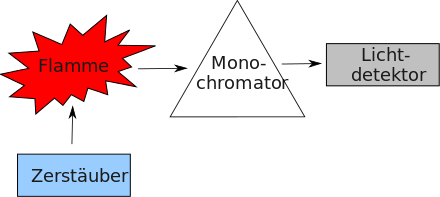
\includegraphics[scale=0.4, center]{images/TheorieAufbauAS.png} 
        %\caption[Schematischer Aufbau eines Atomspektrometers, Quelle: https://www.wikiwand.com/de/\\Atomspektroskopie (Zugegriffen am: 08.01.2020)]{Schematischer Aufbau eines Atomspektrometers}
        %\label{fig:AufbauAtomspektrometer}
      %\end{figure}
      
    
    \subsubsection{Lampe}
    
      Es wird eine Lampe verwendet, die elementspezifisches Licht aussendet (Linienstrahler). In Verwendung sind Hohlkathodenlampen (HKL) und Elektrodenlose Entladungslampen (EDL).
      
      \begin{itemize}
        \item Hohlkathodenlampe: 
        
          HKL bestehen aus einem Glaszylinder (Inertgasfüllung) mit zwei Elektroden - einer Wolfram Anode sowie einer Hohlkathode aus dem zu bestimmenden Element. An der Vorderseite des Glaszylinders befindet sich ein Quarzfenster. Hochspannung zwischen den Elektroden führt zur Ionisierung des Inertgases an der Anode. Im elektrischen Feld werden die positiven Ionen zur Kathode beschleunigt und schlagen dort Atome heraus. Diese werden durch Zusammenstöße mit anderen Gasatomen angeregt und emittieren bei der Relaxation das charakteristische Linienspektrum. Nachteile sind Selbstabsorption bei zu hohen Spannungen sowie Verbrauch der Lampe. Dafür ist das Spektrum linienarm mit sehr schmalen Linien. \citep[S. 84]{AnalytikIII} 
          
                 
        \item Elektrodenlose Entladungslampe:
        
          Das Kernstück der EDL ist eine Quarzkapsel, die mit Inertgas und dem zu bestimmenden Element gefüllt ist. Die Ionisierung des Inertgases erfolgt durch einen Teslafunken im hochfrequenten Wechselfeld. Durch die Erwärmung verdampft das Element und wird angeregt und emittiert bei der Relaxation das charakteristische Linienspektrum. Die Vorteile sind kein Verbrauch des Elements, keine Selbsabsorption sowie höhere Intensitäten als bei der HKL. Allerdings sind nur wenig leicht verdampfbare Elemente (unter \SI[mode=text]{1000}{\degreeCelsius}) verwendbar. Zudem sind die Linien breiter (höhere Temperaturen) und es kommt zur Ionisierung bei zu hohen Feldstärken. \citep{AnalytikIII} 
          
      \end{itemize}
      
    \subsubsection{Atomisator}
    
      Im Atomisator wird die Probe verdampft und anschließend atomisiert. Dabei werden hohe Temperaturen (über \SI[mode=text]{1000}{\degreeCelsius}) benötigt, um die Moleküle und Salze der Probe in die einzelnen Atome zu dissoziieren. Es gibt die Flammen-, Graphitrohr-, Hydrid und Quecksilber Kaltdampf-Technik. Da im Experiment nur die Flammentechnik zum Einsatz kommt, wird auf eine nähere Beschreibung der anderen Techniken verzichtet. \\
      
      Bei der Flammentechnik wird die Probe durch einen Zerstäuber mithilfe des Bernoulli-Prinzips angesaugt und zu kleinen, homogenen Tröpfchen zerstäubt. Die Atomisierung ist dabei umso vollständiger, desto feiner und homogener die Tröpfchen sind. Nach der Zerstäubung wird die Probe in der Flamme getrocknet, verdampft, dissoziiert und angeregt. Für diese Vorgänge sind Temperaturen von \SI[mode=text]{2000}{\degreeCelsius} bis \SI[mode=text]{10000}{\degreeCelsius} nötig. Die Temperatur wird durch die Wahl von Brenngas und Oxidationsmittel reguliert. Bei der AAS ist der Brenner (heutzutage hauptsächlich Laminarbrenner) parallel zum Strahlengang der Lichtquelle ausgerichtet. Dadurch ist die Schichtdicke und Empfindlichkeit am größten. Bei der FES wird der Brenner um \SI[mode=text]{45}{\degree} gedreht. Aufgrund der geringeren Schichtdicke wird die Verringerung der Intensität des emittierten Lichts durch Selbstabsorption und somit eine Abweichung vom linearen Verhalten der Intensitäts-Konzentrationskurve verhindert. Vorteile der Flammen AAS sind Robustheit, einfache Bedien- und Automatisierbarkeit, geringe Störanfälligkeit und ein hoher Probendurchsatz.  Dafür sind sie nicht so empfindlich und benötigen viel Probe aufgrund der geringen Zerstäubereffizienz. \citep{AnalytikIII}
        
    \subsubsection{Monochromator}
      
      Mit dem Monochromator erfolgt die Auswahl einer Wellenlänge, meist die Resonanzlinie, des Spektrums. Die Leistungsfähigkeit des Monochromators ist zusammen mit dem Atomisator maßgeblich für die Qualität der Analyse verantwortlich, insbesondere bei der FES, da das Licht aufgrund der vielen Substanzen in der Probe polychromatischer ist. Durch einen Eintrittsspalt fällt paralleles Messlicht auf ein dispergierendes Element, an dem die Lichtwelle in Abhängigkeit von der Wellenlänge $\lambda$ gebrochen oder gebeugt wird. Prismen beruhen auf dem Prinzip der Brechung. Gitter beruhen auf dem Prinzip der Beugung, besitzen eine höhere Trennleistung und werden deswegen dem Prisma vorgezogen. Sie werden im Folgenden näher beschrieben.
      
      Reflexionsgitter besitzen in regelmäßigen Abständen (in der Größenordnung der Wellenlänge) voneinander getrennte Vertiefungen mit unterschiedlichen Formen, sogenannte Gitterlinien. An diesen Gitterlinien wird die Lichtwelle gebeugt (Huygens'sche Prinzip). Für konstruktive Interferenz der so gebildeten Elementarwellen muss der Wegunterschied $\Delta s$ zweier benachbarter, paralleler Wellen einem ganzzahligen Vielfachen der Wellenlänge entsprechen. Exemplarisch ergibt sich für ein Echellegitter
      
        \begin{equation}
          \Delta s = d \left(\sin i - \sin r\right) = n \lambda,
        \end{equation}
      mit Wellenlänge $\lambda$, Abstand zweier Gitterlinien $d$, Einfallswinkel $i$, Reflexionswinkel $r$ und einer ganzen Zahl $n$ (Winkel zur Gitternormalen gemessen). Die Wellenlänge wird durch Variation des Einfallswinkel ausgewählt. Dies erfolgt unter Verwendung von einem oder zwei Spiegeln (Ebert bzw. Czerny-Turner Aufstellung). \citep{AnalytikIII}
      
    \subsubsection{Detektor}
      
      Der Detektor wandelt elektromagnetische Wellen in ein der Intensität proportionales elektrisches Signal um. Beim verwendeten Photomultiplier werden an der photosensitiven Kathode Elektronen herausgeschlagen (Photoeffekt). Diese werden beim Auftreffen auf die Sekundärelektroden durch stufenweise erhöhte Spannungen vervielfacht und das Signal verstärkt. Wichtig sind gute spektrale Empfindlichkeit, ein breiter linearer Verstärkungsbereich sowie geringes Dunkelrauschen. \citep{AnalytikIII}
      
  \subsection{Störungen beim Messvorgang}
    
    \subsubsection{Chemische Störungen}
    
      Bei chemischen Störungen wird durch Bildung schwer dissoziierbarer Verbindung sowie durch Ionisation die vollständige Atomisierung der Probe verhindert und dadurch die tatsächliche Probenkonzentration verfälscht. Kann durch Verwendung von releasing und protecting agents, Erhöhung der Temperatur sowie mit Ionenpuffern verhindert werden. \citep{AnalytikIII}
  
    \subsubsection{Spezifische und unspezifische spektrale Störungen}
      
      Bei der spezifischen spektralen Störung überlappen die Absorptions- bzw. Emissionslinie(n) der interferierenden Substanz mit der Wellenlänge des Analyten. Bei der unspezifischen spektralen Störung befinden sich undissozierte Verbrennungsprodukte der Probenmatrix im Strahlengang, was zur Streuung des Lichts führt. Die Folge sind Molekülbanden und Breitbandabsorption. Die Auswirkung auf die Messung der Probenkonzentration bei der AAS und FES sind unterschiedlich. Abhilfe kann durch Untergrundkorrektur erfolgen, beispielsweise nach Smith-Hiftje oder Zeemann. \citep{AnalytikIII}
  
      